%!TEX program = xelatex
% Note: this template must be compiled with XeLaTeX rather than PDFLaTeX
% due to the custom fonts used. The line above should ensure this happens
% automatically, but if it doesn't, your LaTeX editor should have a simple toggle
% to switch to using XeLaTeX.

\documentclass[
  aspectratio=169, % Uncomment to use an aspect ratio of 16:9 (160 mm by 90 mm)
  %aspectratio=43, % Uncomment to use an aspect ratio of 4:3 (128mm by 96mm)
  t, % Top align all slide content by default
  onlytextwidth, % Typeset content in columns at text width
  10pt, % Default font size, use 10pt for the 16:9 aspect ratio and 8pt for the 4:3 aspect ratio
]{beamer}

\usepackage{../../ImperialTheme/beamer/beamerthemeImperial} % Use the Imperial theme
\usepackage{tikz}
\usetikzlibrary{calc}

\def\imagefolder{../../ImperialTheme/beamer/Images}
\def\Rey{\text{Re}}
\title{3d stuff + 2d TS waves} % Presentation title to appear on the title slide and left footers

\subtitle{} % Presentation subtitle to appear on the title slide

\author{Víctor Ballester} % Author name(s) to appear on the title slide

\date{\today} % Presentation date to appear on the title slide and right footers

\begin{document}

\begingroup
\setbeamercolor{background canvas}{bg=ICLLightGrey} % Slide background color
\setbeamercolor{title page title}{fg=ICLBlue} % Title text color
\setbeamercolor{title page subtitle}{fg=ICLBlue} % Subtitle text color
\setbeamercolor{author}{fg=ICLBlue} % Author(s) text color
\setbeamercolor{date}{fg=ICLBlue} % Date text color
\setbeamertemplate{title page}[logo]{\imagefolder/ICL_Logo_Blue.pdf} % Imperial logo color, use 'ICL_Logo_White.pdf' for white and 'ICL_Logo_Blue.pdf' for blue
\frame[plain, s]{\titlepage} % Output the title page with no footer ('plain') and vertically distributed text ('s')
\endgroup

\begin{frame}
	\frametitle{Organization Inc work}
	\begin{columns}[T] % [T] ensures correct vertical alignment
		\begin{column}{0.49\linewidth} % left column
			\begin{enumerate}
				\item 2d hopf bifurcation line as a curve in the plane $(w,d)$.
				\item ts mode growth for corroboration of jeff results. good match between ``jeff by pass transition boundary" and hopf bifurcation boudnary, even though one simulation is 2d incns and the other is 3d comns. why? this motivates the 3d analysis.
				\item start 3d linear stability analysis. we find the that for deep gaps the 3d instability happens before the 2d one. but for shallow gaps the 2d instability happens first.
				\item do full 3d (16 complex fourier modes) analysis for different cases:
			\end{enumerate}

		\end{column}
		\begin{column}{0.49\linewidth} % left column
			\begin{figure}[ht]
				\centering
				\includegraphics[width=\textwidth]{Images/stabilitycurvescombined.pdf}
			\end{figure}
		\end{column}
	\end{columns}
\end{frame}
\begin{frame}
	\frametitle{Problems that prevent me to start writing the paper}
	\begin{itemize}
		\item Doing 3d linear stability analysis with only one mode, the 3d modes looks more unstable than the 2d. For example for $d=4$, $w=19$ (after hopf bifurcation boudnary) the simulations outputs a 3d mode (with $w=0$) and growth rate $\simeq 4\cdot 10^{-3}$. 2d LSA give the self-sustained oscilaltion with growth rate $\simeq 2.4 \cdot 10^{-3}$. But in full 3d simulations, after adding small noise to the unstable baseflow, I get first the 2d mode growing with the expected growth rate and expected frequency.
	\end{itemize}
	\begin{columns}[T] % [T] ensures correct vertical alignment
	\begin{column}{0.49\linewidth} % left column
		u isovolumes of 3d mode with $k_z = 2\pi/L_z$ with $L_z = 1.25 d$ (around the most unstable 3d wavenumber). The mode has $w=0$.
		\vspace{-0.5cm}
		\begin{figure}[ht]
			\centering
			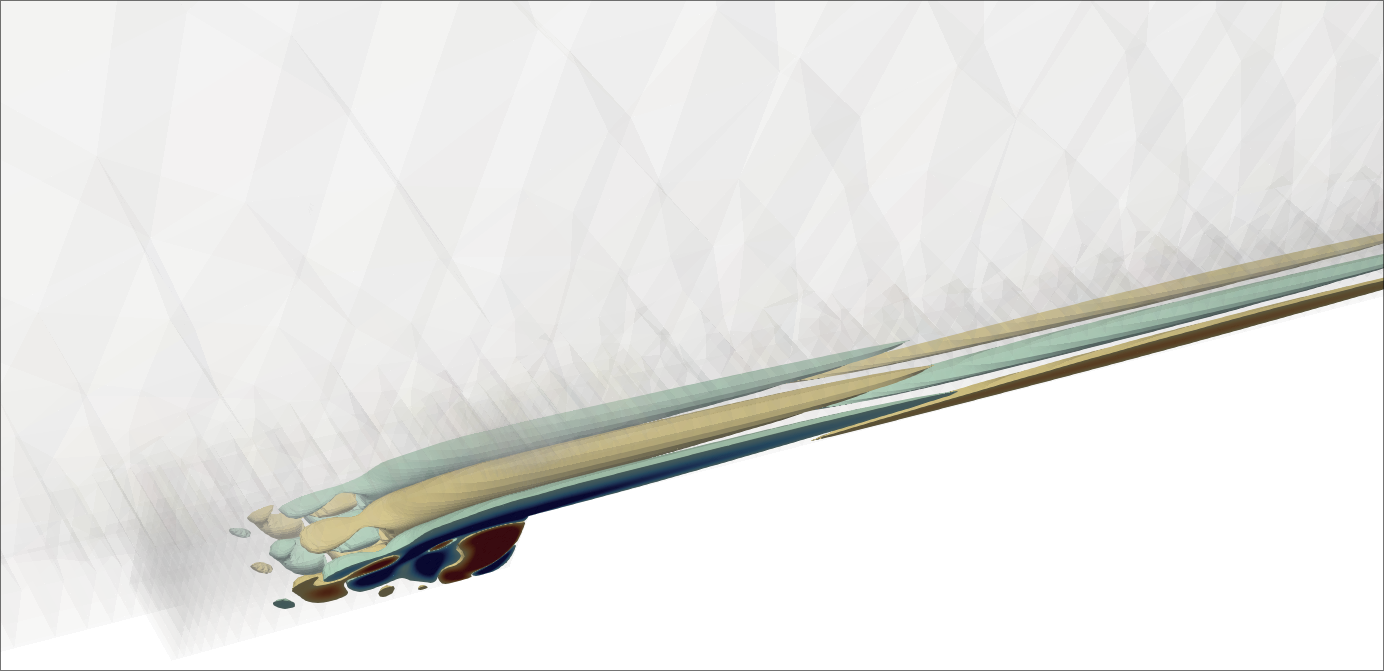
\includegraphics[width=\textwidth]{Images/d4w19_3dmode_u.png}
		\end{figure}
	\end{column}
	\begin{column}{0.49\linewidth} % left column
		$v$ heatmap of the 2d mode with at same $d=4$, $w=19$.
		\begin{figure}[ht]
			\centering
			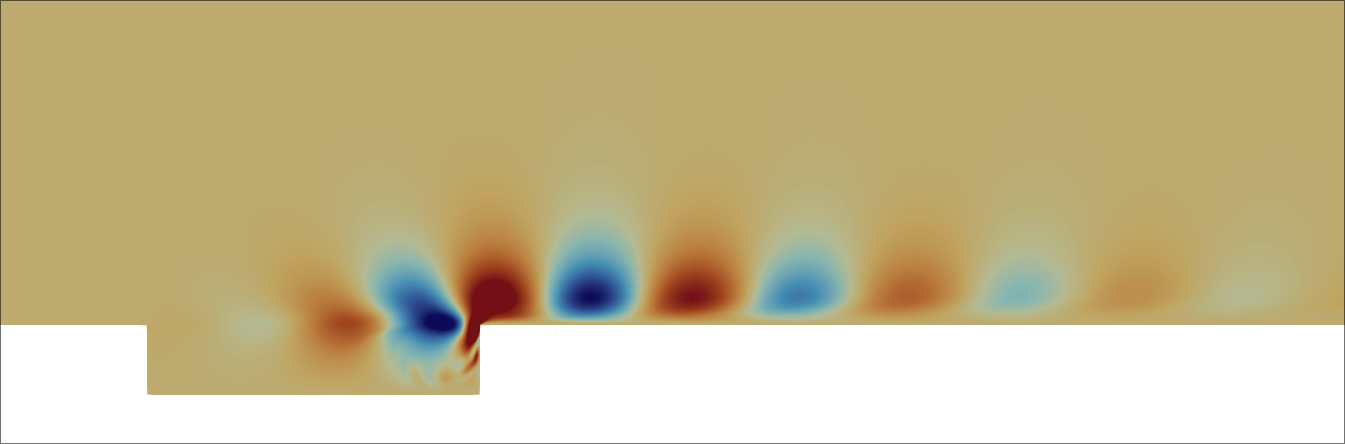
\includegraphics[width=\textwidth]{Images/d4w19_2dmode_v.png}
		\end{figure}
	\end{column}
	\end{columns}
\end{frame}
\begin{frame}
	\frametitle{Parenthesis: SVV consistency}
	SVV modifies quite a lot the growth rate of the most unstable eigenvector in the system.

	For example for $d = 4$, $w = 19$:
	\begin{itemize}
		\item $\sigma_{\text{NO SVV}} = 2.4703 \cdot 10^{-3}$, $\omega_{\text{NO SVV}} = 0.24573$
		\item $\sigma_{\text{SVV}} = 2.6004  \cdot 10^{-3}$, $\omega_{\text{SVV}} = 0.24594$
		\item Relative error in $\sigma$ is $5.2\%$, while in $\omega$ is $0.08\%$
		\item The growth rate with SVV matches the one of 3d dns (because there I have SVV activated as well) up to less than 1\% error. And the frequency even better.
	\end{itemize}

\end{frame}
\begin{frame}
	\frametitle{Problems that prevent me to start writing the paper}
	\begin{itemize}
		\item For a shallow gap case, like $d=1.5$, $w=70$, after DNS finishes the transient state, it stabilizes into a time-periodic signal with the $\omega_{DNS} \approx 0.116$. However when running 2d LSA, I obtain two unstable modes (at least), each of different frequency: $\omega_1 \approx 0.157$ ($\sigma_1 \approx 0.00368$) and $\omega_2 \approx 0.119$ ($\sigma_2 \approx 0.00237$). So there is an interaction between the two modes that do not produce chaos yet. 
	\end{itemize}
		\vspace{-0.3cm}
		Limit cycle of nonlinear simulation for $d=1.5$, $w=70$. $v$ contours.
		\vspace{-0.5cm}
		\begin{figure}[ht]
			\centering
			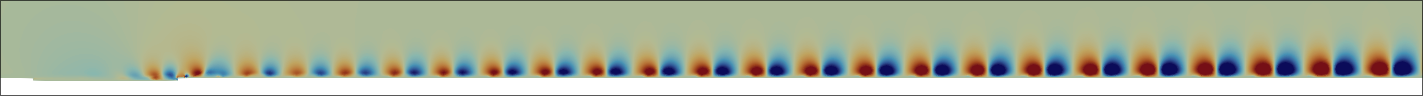
\includegraphics[width=\textwidth]{Images/d1.5w70_DNS_po.png}
		\end{figure}
		\vspace{-0.5cm}
		Most unstable 2d mode for $d=1.5$, $w=70$. $v$ heatmap.
		\vspace{-0.5cm}
		\begin{figure}[ht]
			\centering
			
\includegraphics[width=\textwidth]{Images/d1.5w70_mode1.png}
			\end{figure}
		\vspace{-0.5cm}
		Second most unstable 2d mode for $d=1.5$, $w=70$. $v$ heatmap.
		\vspace{-0.5cm}
		\begin{figure}[ht]
			\centering
			
\includegraphics[width=\textwidth]{Images/d1.5w70_mode2.png}
		\end{figure}
\end{frame}
\begin{frame}
	\frametitle{Transition process at $d=1.5$, $w=80$ (TS mode transition)}
\begin{figure}[ht]
			\centering
			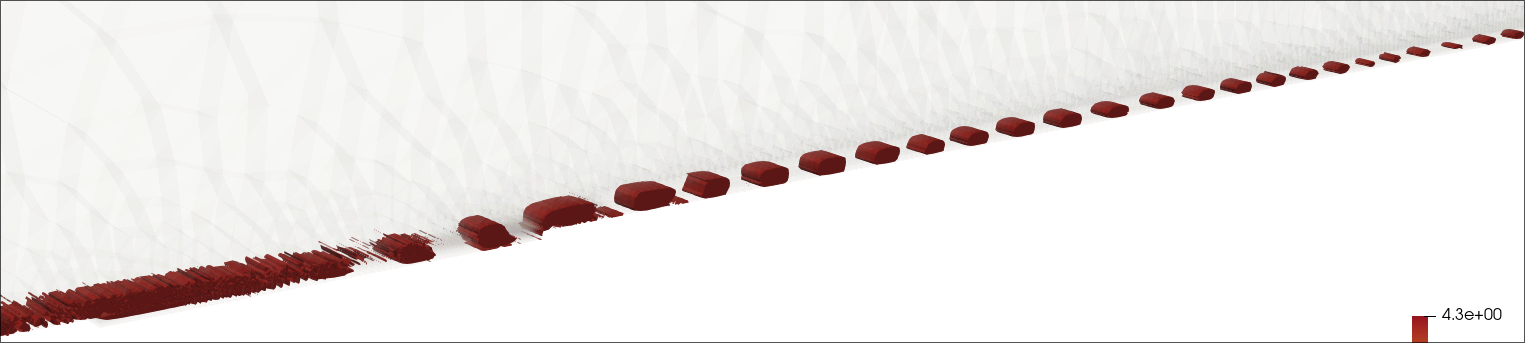
\includegraphics[width=\textwidth]{Images/d1.5w80_trans1.png}
		\end{figure}
\end{frame}
\begin{frame}
	\frametitle{Transition process at $d=1.5$, $w=80$ (TS mode transition)}
\begin{figure}[ht]
			\centering
			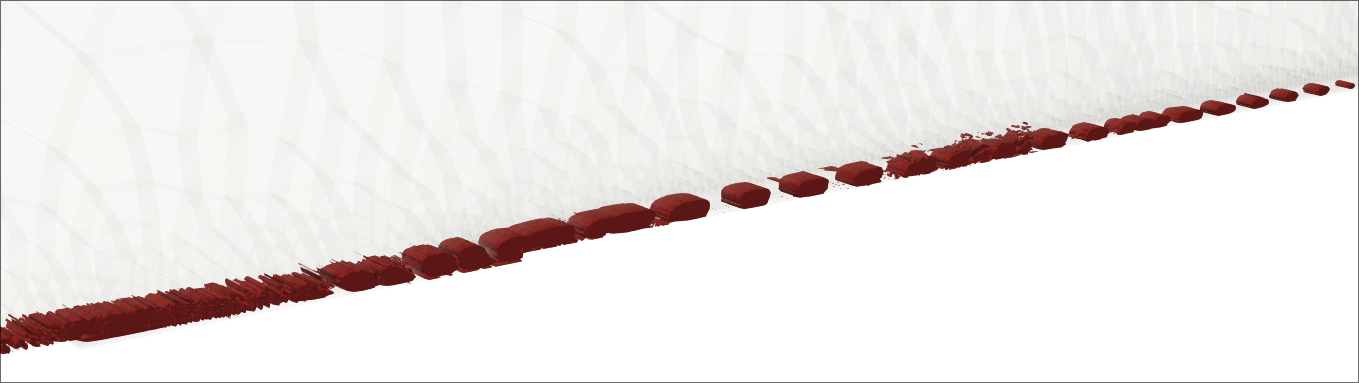
\includegraphics[width=\textwidth]{Images/d1.5w80_trans2.png}
		\end{figure}
\end{frame}
\begin{frame}
	\frametitle{Transition process at $d=1.5$, $w=80$ (TS mode transition)}
\begin{figure}[ht]
			\centering
			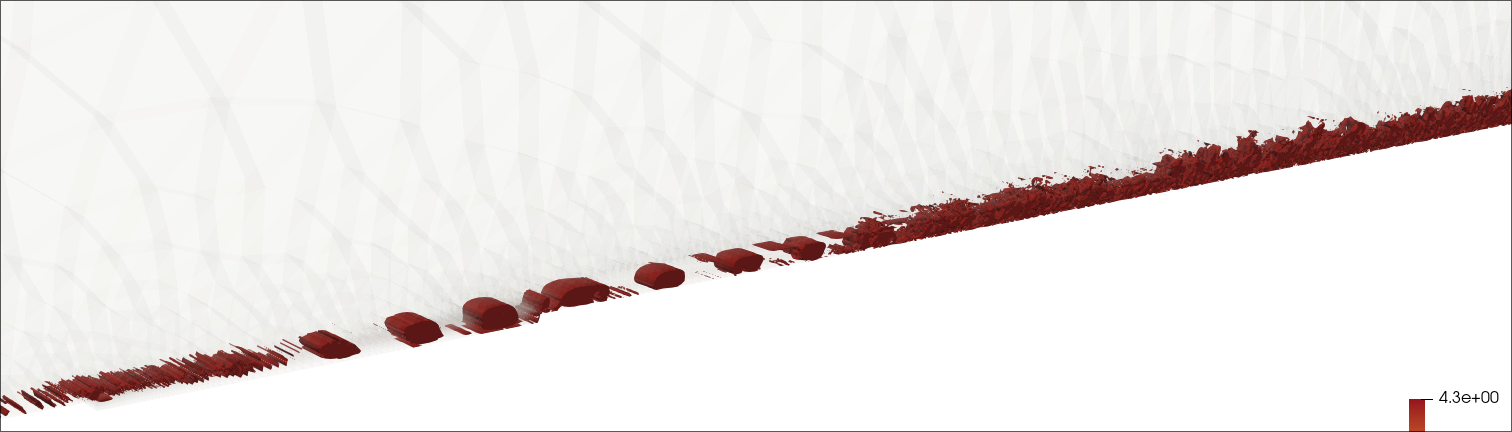
\includegraphics[width=\textwidth]{Images/d1.5w80_trans3.png}
		\end{figure}
\end{frame}
\end{document}
